% E3 paper figure (bidirectional 7 x 7 benchmark): wbc_coordination.pdf
% PDF: 515.5 x 212.4 pt = 7.16 x 2.95 in = \textwidth; insert at 100 % scale.
% Fonts: STIX (Times-compatible), embedded TrueType. DRAFT caption -- not yet inserted
% into the manuscript. Numbers: E3_REPORT.md / stats/.

\begin{figure*}[t]
    \centering
    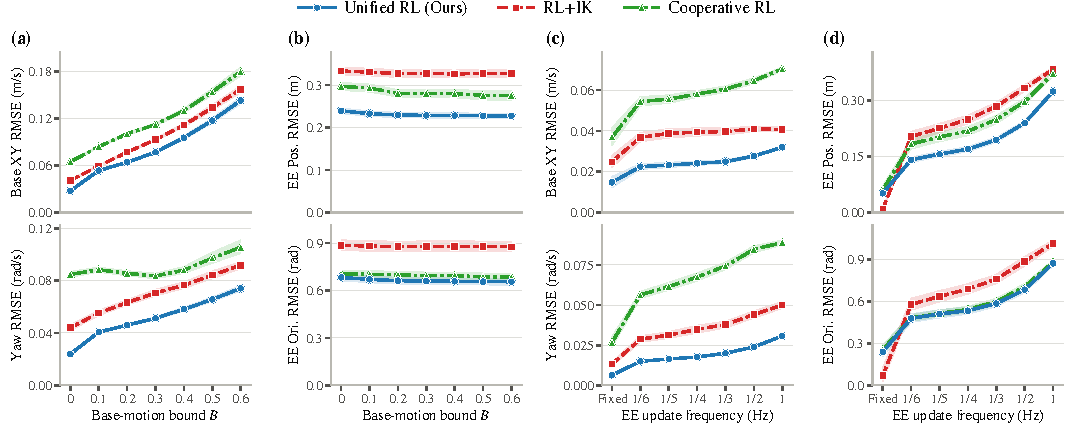
\includegraphics[width=\textwidth]{figures/wbc_coordination.pdf}
    \caption{Bidirectional whole-body tracking. Base commands are piecewise constant
    within the symmetric bound $B$ on planar velocity (m/s) and yaw rate (rad/s); EE
    targets are full 6-DoF poses drawn from the training pose set and switched without
    interpolation at the given update frequency (``Fixed'' holds one target).
    (a)~Base XY velocity (top) and yaw-rate (bottom) RMSE and (b)~EE position (top) and
    orientation (bottom) RMSE versus $B$, with EE updates at 1/2\,Hz.
    (c)~Base and (d)~EE tracking RMSE versus EE update frequency with a stationary base
    command ($B=0$). (a)--(b) and (c)--(d) each share the same trials. RMSEs are computed
    over 3--30\,s, including transients after command updates. Lines are means over 100
    paired simulation trials; bands are 95\% bootstrap confidence intervals of the mean.}
    \label{fig:wbc_coordination}
\end{figure*}
